\documentclass[tikz,border=12pt]{standalone}
\usepackage{amsmath}
\usepackage{amssymb}
\usepackage{tikz}
\usetikzlibrary{arrows.meta}

\definecolor{ink}{HTML}{0F172A}
\definecolor{linegray}{HTML}{64748B}
\definecolor{inputfill}{HTML}{F8FAFC}
\definecolor{outputfill}{HTML}{CBD5E1}

\begin{document}
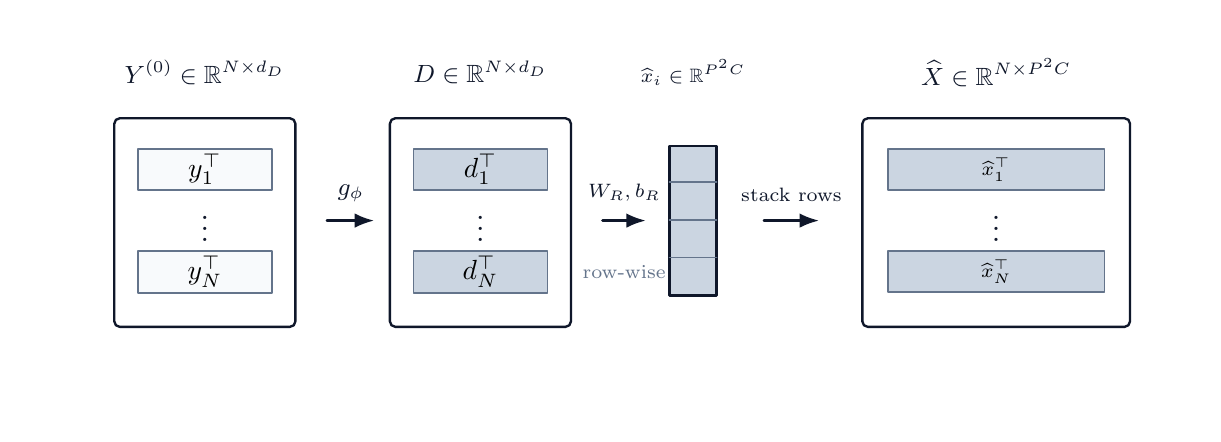
\begin{tikzpicture}[
  font=\sffamily,
  >=Latex,
  line cap=round,
  line join=round,
  row/.style={
    draw=linegray,
    line width=0.6pt,
    minimum height=0.52cm,
    inner sep=2pt,
    align=center
  },
  matrix box/.style={
    draw=ink,
    line width=0.85pt,
    rounded corners=2pt,
    inner sep=0pt
  }
]
  \fill[white] (-0.6,-0.75) rectangle (14.2,4.15);

  % Decoder input.
  \node[ink, font=\small] at (1.65,3.58)
    {$Y^{(0)} \in \mathbb{R}^{N\times d_D}$};
  \draw[matrix box] (0.5,0.35) rectangle (2.8,3.0);
  \node[row, fill=inputfill, minimum width=1.7cm] at (1.65,2.35)
    {$y_1^\top$};
  \node[ink, font=\large] at (1.65,1.7) {$\vdots$};
  \node[row, fill=inputfill, minimum width=1.7cm] at (1.65,1.05)
    {$y_N^\top$};

  % Decoder transformer.
  \draw[ink, ->, line width=0.9pt]
    (3.2,1.7) -- (3.8,1.7)
    node[midway, above=5pt, fill=white, inner sep=1.5pt, font=\small]
      {$g_\phi$};

  \node[ink, font=\small] at (5.15,3.58)
    {$D \in \mathbb{R}^{N\times d_D}$};
  \draw[matrix box] (4.0,0.35) rectangle (6.3,3.0);
  \node[row, fill=outputfill, minimum width=1.7cm] at (5.15,2.35)
    {$d_1^\top$};
  \node[ink, font=\large] at (5.15,1.7) {$\vdots$};
  \node[row, fill=outputfill, minimum width=1.7cm] at (5.15,1.05)
    {$d_N^\top$};

  % Apply the reconstruction projection to each decoder row.
  \draw[ink, ->, line width=0.9pt]
    (6.7,1.7) -- (7.25,1.7)
    node[midway, above=5pt, fill=white, inner sep=1.5pt, font=\scriptsize]
      {$W_R,b_R$};
  \node[linegray, font=\scriptsize] at (6.975,1.05)
    {row-wise};

  \node[ink, font=\scriptsize] at (7.85,3.58)
    {$\widehat{x}_i \in \mathbb{R}^{P^2 C}$};
  \draw[ink, line width=0.9pt, fill=outputfill]
    (7.55,0.75) rectangle (8.15,2.65);
  \draw[linegray, line width=0.55pt] (7.55,1.23) -- (8.15,1.23);
  \draw[linegray, line width=0.55pt] (7.55,1.71) -- (8.15,1.71);
  \draw[linegray, line width=0.55pt] (7.55,2.19) -- (8.15,2.19);

  % Stack the reconstructed patches.
  \draw[ink, ->, line width=0.9pt]
    (8.75,1.7) -- (9.45,1.7)
    node[midway, above=5pt, fill=white, inner sep=1.5pt, font=\scriptsize]
      {stack rows};

  \node[ink, font=\small] at (11.7,3.58)
    {$\widehat{X} \in \mathbb{R}^{N\times P^2 C}$};
  \draw[matrix box] (10.0,0.35) rectangle (13.4,3.0);
  \node[row, fill=outputfill, minimum width=2.75cm, font=\scriptsize]
    at (11.7,2.35) {$\widehat{x}_1^\top$};
  \node[ink, font=\large] at (11.7,1.7) {$\vdots$};
  \node[row, fill=outputfill, minimum width=2.75cm, font=\scriptsize]
    at (11.7,1.05) {$\widehat{x}_N^\top$};
\end{tikzpicture}
\end{document}
